\chapter{Timestamping}
\label{chpr:timestamping}
Placing a certain date on some data is surprisingly useful \cite{Haber91howto, Bayer93improvingthe, Massias99designof, OTSannouncment}.
An inventor who had a patentable idea or a scientist who came to a relevant conclusion may want to create a verifiable proof that at a certain moment they discovered something. This can help them to protect their intellectual property, proving others their precedence over competing claims.
In a communication protocol having the possibility to attach a certain time to messages can improve the security of the transmission. However it is often difficult to come to an agreement on which is the correct time to use, so different security models yield to different practical schemes.
When storing documents in a third party cloud server, it could behave maliciously, for instance modifying their contents. Placing a certain and tamper resistant date on a document will make harder for the server provider to corrupt that file: the attacker should also be able to falsify the certificate stating the date. 

Other practical applications of this technique are possible, however to have a complete understanding of the subject it is important to figure out which are its limits and which are the right choices to take to correctly put the concepts into practice. So we need to be a little more formal,
\begin{mydef}
	A timestamp is a proof that some data $d$ existed prior to time $t$.
\end{mydef}
To create such proof, $d$ has to cause an event that could not have been generated without the existence of $d$. Such event it is bound to time $t$ and can be observed by others, we call its record \textit{time attestation}. So a proof consists in the data $d$, the set of \textit{operations} that were applied to cause the event and the time attestation.

Proofs are useful if they are able to convince the verifiers. He must be able to check the correctness of the operations and must retain trustworthy the time attestation. Depending on the problem in exam one should properly choose which operations and attestations to use. 

Let's consider the case of a sent letter. The data $d$ is the content of the letter, $d$ caused the palpable letter: if $d$ were different the letter would be different. When the letter went through the post office a postmark with the date $t$ was stamped on the letter, the postmark is the time attestation. If the post officer is trustworthy, a verifier who examines the letter may be convinced that the content of the letter existed prior to the time stated in the postmark. However a good counterfeiter could change the content of the letter or falsify the postmark placing a false date, thus for some cases such proof would not be appropriate.

In the case of a digital document new problems arises: it is not necessary to be a good counterfeiter to falsify a document without leaving any kind of tamper evidence, thus new solutions must be adopted. A timestamp for the data $d$ should guarantee that if even only a single bit of $d$ is modified the timestamp proof becomes invalid. To solve this problem cryptography tools are used \cite{Haber97securenames}. Digital data can also be shared easily and with little costs, this is among the features that enables the possibility to achieve distributed and decentralized consensus. Such an achievement would give user the chance to timestamp without any trust in a third party.

Resuming, at a certain moment $t_e$ some data $d$ exists, then at $t_c$ someone (or something) will have the necessity to prove the existence of $d$, so he implements the timestamp \textit{creation procedure} that results in a proof stating that $d$ existed priort to time $t$. Consequently at time $t_v$ a challenger implements the \textit{verification procedure} that ends in a binary result: true if he retains the proof correct, false otherwise. Naturally we have $t_e<t_c<t<t_v$.

To avoid common misunderstandings, it is important to clarify what a timestamp does not prove. The time $t$ is the first moment when $d$ went to existence, the creation procedure is not instantaneous and of course if the proof for $(d,t)$ is true then there exists a proof for $(d,t')$ which holds true for all $t'>t$. A timestamp is not necessarily linked to its creator and moreover it doesn't prove that who owns the timestamp (it can be owned by multiple entities) is the creator of the data $d$: it just proves that someone knew $d$. If an inventor comes up with a timestamp stating that he had a particularly smart idea prior to time $t$, it does not mean that he was the first one to have such idea, in fact he could have simply overheard the idea from a colleague and afterwards timestamped it. A timestamp does not prove that data $d' \neq d$ does not exist. Imagine someone stating that he knew the result of the elections prior to the vote, he provides a timestamp and claims that it proves he predicted the correct outcome. However he could be an imposter: he may had timestamped several different results and once he saw how the vote count ended he will provide only the proof which make him look as a visionary.
Although these limitations being able to timestamp is still useful. If stronger proofs are needed the used system must be endowed with other tools that actually provides what is asked. 

In the following sections we analyse the two ingredients of timestamp proofs: operations and attestations.

\section{Commitment Operations}

The operations that compose a timestamp proof should be defined in a precise way, a verifier will check their correctness when evaluating the proof. An useful operation binds the data in a way that it is hard or impossible to modify the data after the creation of the timestamp. Being more general, such an operation commits the input to the output: the input cannot be changed without changing the output. The result of the operation is a commitment to the input, in the sense that it was caused by the input or, in other words, the input precede in time the output.
For instance in the case of a sent letter, the input is the content of the letter, the piece of paper that is sent is the output and physically writing the letter is the operation that commits the input to the output. We can say that a letter is a physical commitment to its content. If one wants to modify the content of the letter ex post it will change the letter itself. However, tamper evidence could be extremely hard to spot.

Digital document are easier to tamper, but they could be defined in a more precise way, representing each document with bits. To take full advantage of this, we need a formal definition,
\begin{mydef}
	A function $C:X \rightarrow Y$ is a commitment operation if given $x_1 \in X$ it is not feasible to compute $x_2 \in X$ s.t. $x_1 \neq x_2, C(x_1)=C(x_2)$.
\end{mydef}
The property required is sometimes referred as second pre-image resistance. For practical purposes $X$, $Y$ can be thought as bit string spaces, their element can be seen as bit strings or another of their representations, for instance in hexadecimal digits or using a conventional encoding.
The simplest examples are the append and prepend operations:

\begin{myexample}
	\textquotedblleft hello\textquotedblright $\xrightarrow{\text{append(\textquotedblleft world\textquotedblright)}}$ \textquotedblleft helloworld\textquotedblright.
\end{myexample}
It is impossible to change the input without changing the output: the output contains the input itself. In this example the function is a unary operation, since it takes only one input, however commitment operation may have more than one input:
\begin{myexample}
	\textquotedblleft world\textquotedblright, \textquotedblleft hello\textquotedblright $\xrightarrow{\text{prepend()}}$ \textquotedblleft helloworld\textquotedblright.
\end{myexample}
Append and prepend have two problems: they reveal everything about the inputs and the size of the output is always greater than the size of the inputs. 

Hiding the input of a commitment is often useful. For instance Robert Hooke \cite{Petroski96invention} in 1676 had formulated the spring law that will take his name. He wanted to prove that he knew that without revealing the law itself, so he published the latin anagram \textquotedblleft ceiiinosssttuv\textquotedblright. Later in 1678 he revealed the solution, \textquotedblleft ut tensio, sic vis\textquotedblright (\textquotedblleft as the extension, so the force\textquotedblright). However the anagram is not an optimal commitment operation: \textquotedblleft ut vis, sic tensio\textquotedblright is a solution too. For that time it was an acceptable solution, the verification procedure had minimal requirements and there was no real incentive in lying. Nowadays better solutions are available, hence using an anagram will make the verifier suspicious.

To address this problems cryptographic hash functions are used. Hash functions maps bit strings of arbitrary finite length into bit strings of fixed length \cite{Damgard:1989:DPH:118209.118248}. 
\begin{mydef}
	$h : \{ 0, 1 \} ^* \rightarrow \{ 0, 1 \} ^n $ is a hash function if it is computable in polynomial time in the length of the input.
\end{mydef}
We will refer at the input of such functions as preimage, and the output as hash value. The codomain is strictly contained in the domain hence the presence of collisions (pairs of inputs with identical outputs) is unavoidable. 
To give to these functions a practical use some of the following properties are required
\begin{mydef}
	\label{hash-prop}
	Let $h$ be a hash function, the following properties may hold:
	\begin{itemize}
		\item preimage resistance: given $h(x)$ it is not feasible to compute $x$;
		\item second-preimage resistance: given $x$ it is not feasible to compute $y$ s.t. $x \neq y$, $h(x)=h(y)$;
		\item collision resistance: it is not feasible to find $x, y$ s.t. $x \neq y$, $h(x)=h(y)$.
	\end{itemize}
\end{mydef}

A preimage resistant hash function hides the inputs, this property is sometimes referred as one-wayness.
A second-preimage resistant hash function is also a commitment operation, in addition it hides the input and create a fixed size fingerprint. A huge file can be mapped into a short bit string which is a commitment to it.
Collision resistance, although is a nice to have, is not necessary for timestamping purposes: when a collision ($x \neq y$ s.t $h(x)=h(y)$) is found, $x$ and $y$ are found at the same time \cite{SHA1}.

Such properties depend on the dimension of the codomain, which is given by the parameter $n$, precisely $2^n$. If it is too low it will be easy to produce examples that invalidates the properties, if it is too high the hash function is not a good tool for reducing the size of the input. A good compromise has to be found, it should be based on the current state of the art of cryptanalysis and computer science. However what is considered acceptable during a period may not be accepted in a subsequent one, in fact if new techniques that break an hash function are discovered, then its use will be considered insecure.
Several hashing functions has been proposed, we show a couple of examples:
\begin{myexample}
	SHA1 (Secure Hashing Algorithm) was designed by the National Security Agency (NSA), and released in 1995. It maps bit strings to a 160 bit space, it was considered preimage, second-preimage and collision resistant. In 2005 cryptanalysts discover a procedure to find collisions, hence it was declared insecure. However only collision resistance was broken, thus, for it can still be used for timestamping purposes.
	\begin{verbatim}
	SHA1(b'Hello World!\n') = a0b65939670bc2c010f4d5d6a0b3e4e4590fb
	                          92b
	SHA1(b'Hello World\n')  = 648a6a6ffffdaa0badb23b8baf90b6168dd16
	                          b3a
	\end{verbatim}
\end{myexample}

\begin{myexample}
	SHA256 belongs to the family SHA2, the generation of hash functions following SHA1. It outputs  strings 256 bit long and, at the moment, it is considered to satisfy all the properties in Definition \ref{hash-prop}.
	Several systems are built upon this assumption. 
	In addition, as other hash functions, SHA256 could be modeled as a random oracle, a fixed input will provide always the same output, since hash functions are deterministic, but the outputs corresponding to new inputs will give a results, that for someone with a reasonable amount of computing power, are indistinguishable from a uniform distribution. 
	Note how a little change in the input produces outputs very dissimilar in both hash functions, this feature helps to spot alterations in the inputs.
	\begin{verbatim}
	SHA256(b'Hello World!\n') = 03ba204e50d126e4674c005e04d82e84c21
	                            366780af1f43bd54a37816b6ab340
	SHA256(b'Hello World\n')  = d2a84f4b8b650937ec8f73cd8be2c74add5
	                            a911ba64df27458ed8229da804a26
	\end{verbatim}
	Since SHA256 is available, the use of SHA1 should be avoided unless there is a particular motivation. 
\end{myexample}

More complex commitment operations are possible.
But they should be used only if there are some valid and shared motivations. Finding a badly motivated commitment operation in a proof will make verifiers suspicious.

Combining the examples we saw it is possible to implement a data structure that is useful to embed several commitments into a single hash value, 
this structure is called \textit{Merkle tree} [Mer]. Let $h$ be a second-preimage resistant hash function, start from $k$ data to timestamp $\{d_i\}_{i=1}^k$, called \textit{leaves}, compute their hash values $\{h(d_i)\}_{i=1}^k=\{h_i\}_{i=1}^n$. The first step combines the couples of adjacent values (if there is one) by concatenating ($||$) the two values and computing the hash value of the concatenation: $h(h_i||h_{i+1})$ $\forall i \in [1,k]$ odd. The following steps proceed in an analogous manner, but starting from the results computed at the step before as described in Algorithm \ref{alg:merkle-tree}. 

\begin{algorithm}
	\caption{Merkle tree construction}
	\label{alg:merkle-tree}
	\begin{algorithmic}[1]
		\Procedure{merklestep}{$\{h_i\}_{i=1}^k$}
		\State $S \gets \{\}$
		\For {$i\gets 1,k$ s.t. $i\equiv 1 (2)$}
		\State $S \gets S \cup \begin{cases} 
		h(h_i||h_{i+1}) & i \neq k \\ 
		h(h_i) & i=k           
		\end{cases}$
		\EndFor
		\State \textbf{return} $S$
		\EndProcedure
		\Statex
		\Procedure{merklelize}{$\{d_i\}_{i=1}^k$} \Comment{from the leaves to the Merkle tip}
		\State $S \gets \{\}$
		\For {$i\gets 1, k$}
		\State $S\gets S \cup h(d_i)$\Comment{hash the leaves}
		\EndFor
		\State $k\gets |S|$
		\While {$k \neq 1$}
		\State $S \gets$ \Call{merklestep}{S} \Comment{if necessary, store $S$}
		\State $k\gets |S|$
		\EndWhile
		\State \textbf{return} $S$ \Comment{Merkle tip}
		\EndProcedure
	\end{algorithmic}
\end{algorithm}

After at most $\lceil log(k) \rceil$ steps the algorithm ends and one hash value is returned, it is called \textit{Merkle tip} or \textit{Merkle root}. 
Thanks to reiteration of $h$ the tip is a commitment to all the leaves $\{d_i\}_{i=1}^k$, moreover to prove that a element $d_i$ is committed it is not necessary to know all tree, in fact it's enough to show the \textit{Merkle path} starting from $d_i$ and ending in the tip. 
For instance referring to Figure \ref{fig:merkle-tree} the minimal requirement to show the commitment of $data3$ in $MT$ is the ordered sequence of operations to apply is:
\begin{verbatim}
h, append(h4), h, prepend(A), h, append(E), h
\end{verbatim}
Merkle trees can aggregate several commitments into one hash value, giving a scalability solution: the length of a single proof grows logarithmically with the number of leaves.

\begin{figure}
	\begin{center}
		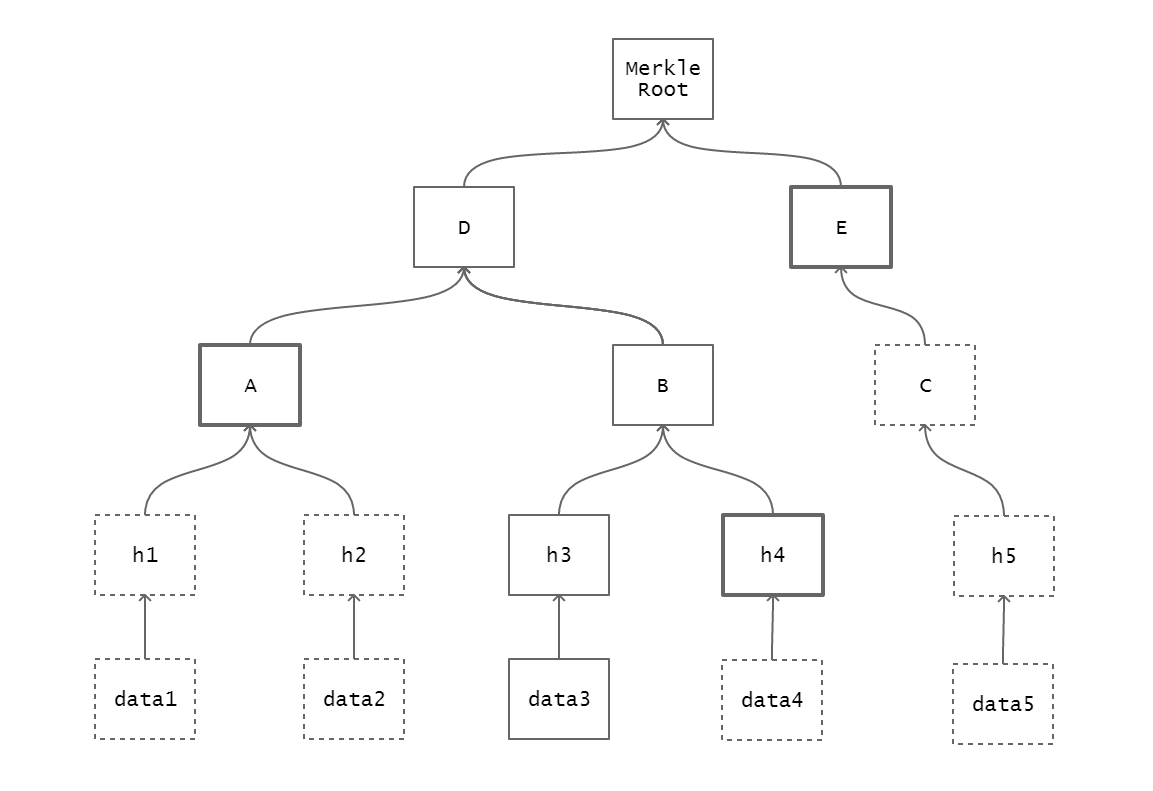
\includegraphics[width=\linewidth]{Images/merkle-tree.png}
		\caption[Merkle tree example]{Merkle tree example. the Merkle root is a commitment to the leaves $\{data_i\}_{i=1}^5$.}
		\label{fig:merkle-tree}
	\end{center}
\end{figure}

\section{Time Attestations}

Attestations are provided by a notary, which has the authority to state the time.
Notaries are sometimes referred as timestamp servers, who ask for creating or verifying that a timestamp is referred as client.
A time attestation binds some data $d$ to the time $t$, $d$ could be directly the data to timestamp or a commitment to them. 

An attestation should be \textit{tamper resistant} or, even better, \textit{immutable}. Once created no one should be able to modify that, backdating the timestamp or changing the underlying data without making the attestation invalid.

In the case of a sent letter an important issue comes to the attention: the attestation (postmark) can be verified only if the letter is in our hands. This makes the task of a counterfeiter easier, few people will examine the postmark making the success of the attack more likely. A solution that mitigates this issue is \textit{widely publishing} the attestation, for instance inserting it in a newspaper. The attacker has an harder task, in most cases, to guarantee himself good chances of success he needs to modify several, or even all, attestations leading to a higher cost. Considering an attestation on a newspaper, an attacker could counterfeit only the exact copy the verifier is going to check. To prevent such situation the verifier should check multiple sources and should not expose any information on where he is retrieving the copies used to examine. Attestations should be \textit{easily accessible}, for instance a good solution is to publish them on the internet.

We call the service providing the attestations notary, it has the authority to state the time. To maintain such power it has to show itself as \textit{trustworthy}: it should place the correct time in the attestations, it should not trick the clients modifying the timestamp ex post and he should not collude with the creator of the timestamp to trick a verifier. Moreover a notary should be \textit{competent}: if it looses the information necessary to verify the timestamp, then its creator will be damaged.

A good notary does not make distinctions among clients or data to timestamp, in other words it does \textit{not censor}. An improvement would be if it is not aware of what it is timestamping, like the case of the commitments hiding their inputs, but even better if it is not aware of being used as a timestamp server, like the newspaper.

In the case of a sent letter, the notary is the post officer, he will place the postmark on the letter giving it a date. 
Clients must trust such notary, which in theory can place a wrong date $t'$ instead of $t$, creating a false timestamp (if $t'<t$) or a deliberate weaker proof (if $t'>t$). Alternately he can decide not to timestamp a letter or modifying its content before timestamping. In addition the resulting timestamp is unique, thus if it gets damaged or lost the proof is gone forever.

A notary willing to show himself as more trustworthy can make its possibly dishonest behaviour harder to implement. A possible solution is to link all the timestamps so that changing one would implies changing all the subsequent ones. A timestamp proof $TS_i$ for the data $d_i$ at the time $t_i$ ($t_{i-1}<t_i<t_{i+1}$) would be something like:
\begin{equation}
	\label{singed-chain}
	\begin{cases}
		TS_0 =(d_0,t_0), \sigma_N((d_0,t_0)) & 
		\\
		TS_i =(d_i,t_i,TS_{i-1}, \sigma_N((d_i,t_i,TS_{i-1}))) & i = 1, ..., i_{max}		
	\end{cases}
\end{equation}
where $\sigma_N (x)$ is a commitment to the data $x$. Such commitment is created by the notary, who is (supposedly) the only one who is able to apply $\sigma_N$. We call this function \textit{signature}, it can be physical (as a postmark) or digital (with a public key cryptosystem). The signature $\sigma_N$ is a commitment operation, so if $TS_{i}$ changes then $\sigma_N((d_{i+1},t_{i+1},TS_i))$ changes, thus $TS_{i+1}$ changes resulting in $TS_j$ changing for all $j>i$. Starting from the \textit{genesis timestamp} $TS_0$, the linked timestamps $\{ TS_{i} \}_{i=0}^{i_{max}}$ form a \textit{chain}. A trusted notary which implement this scheme will be preferred by honest clients. Depending on each particular problem the designer of the system has to properly choose how to collect the timestamp requests, how to commit them into the chain, the time frequency, the signature procedure, how to publish the chain and how to distribute the timestamp proof to the clients.

Even though linking the timestamps is a great improvement with respect to the previous schemes, having a trusted notary still involves some issues. The notary may loose what he needs for signing (e.g. stamp, private key); if an attacker can sign in the place of the notary, it will no longer be considered authoritative; if no one can sign the clients will be damaged. In addition the notary can create more than one chain starting from the same genesis timestamp, then he can use different chains for different clients. 
Anyhow nothing can guarantee that a trusted notary will behave honestly in the future, it can attack some clients in several ways and such bad behaviour can be hard to spot rapidly, a single client may realize that he has been tricked only when he needs the timestamp.

Trusted attestations has security issues hence, in some situations, they could be considered not enough appropriate, yet for years an efficient solution that does not involve a trusted third party was considered barely impossible. 
In 2008 Satoshi Nakamoto proposed \cite{Nakamoto_bitcoin:a} which described a system to transfer value from one party to another without relying on the presence of a central authority. The system can be also used to timestamp arbitrary data without trusting any notary.